% SC4063 --- Chapter 4: VPNs and Secure Tunnelling (0->100)
\chapter{VPNs and Secure Tunnelling}\label{ch:vpn}
\sloppy

\begin{quote}
\emph{``A VPN is a private road painted on a public map.''} --- Packets still
cross the Internet, but observers see only the outer envelope; the inner letter
is sealed and addressed to a private destination.
\end{quote}

\noindent\fbox{\parbox{\dimexpr\linewidth-2\fboxsep-2\fboxrule}{%
\textbf{From zero: envelopes inside envelopes.} We start from a plain IP packet,
wrap it in a new envelope (tunnel), seal it with authenticated encryption, and
negotiate the sealing key. Intuition (postal tunnel) $\to$ encapsulation $\to$
key exchange $\to$ live config. No prior VPN knowledge assumed.}}
\vspace{0.4em}

\section*{Learning Outcomes}
After this chapter you will be able to:
\begin{enumerate}[label=(L\arabic*)]
    \item explain tunnel vs.\ transport encapsulation and the need for a security association;
    \item describe IPsec ESP/AH, IKEv2, and the TLS VPN alternative;
    \item describe WireGuard's Noise handshake and why it is simpler;
    \item choose split vs.\ full tunnel, remote-access vs.\ site-to-site, and kill-switch policy;
    \item audit a VPN for DNS, IPv6, and reconnection leakage and reason about overhead.
\end{enumerate}

% ============================================================
\section{Why Tunnel at All?}\label{sec:why-tunnel}
A private network (10.0.0.0/8) is not routable on the public Internet. A
\emph{VPN} creates a virtual point-to-point link over that public network by
\emph{encapsulating} and \emph{encrypting}. Routing decides what enters the
tunnel; cryptography ensures outsiders see only ciphertext and the outer
headers. Think of putting the entire letter, with its original envelope,
inside a new outer envelope addressed gateway-to-gateway.

\begin{definition}[Security association]\label{def:sa}
A \emph{security association} (SA) is simplex state for one direction:
encryption/integrity algorithms, keys, sequence counter, anti-replay window,
and lifetime. IPsec needs two SAs per flow (inbound/outbound); rekeying
before expiry preserves forward secrecy of the data channel.
\end{definition}

\begin{figure}[h]\centering
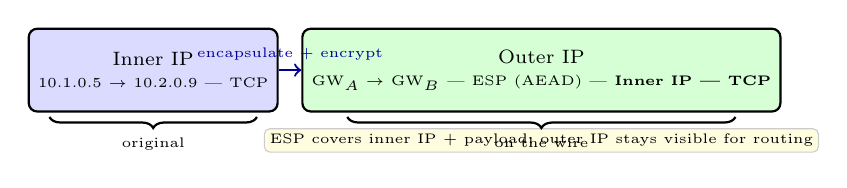
\begin{tikzpicture}[scale=0.85, every node/.style={font=\scriptsize},
  pkt/.style={draw,thick,rounded corners=3pt,minimum height=1.05cm,align=center}]
\node[pkt,fill=blue!14,minimum width=3.0cm] (inner) at (0,0) {Inner IP\\\tiny 10.1.0.5 $\to$ 10.2.0.9 | TCP};
\node[pkt,fill=green!16,minimum width=5.6cm] (esp) at (5.8,0) {Outer IP\\\tiny GW$_A \to$ GW$_B$ | ESP (AEAD) | \textbf{Inner IP | TCP}};
\draw[->,thick,blue!60!black] (inner) -- (esp) node[midway,above,font=\tiny] {encapsulate + encrypt};
\node[font=\tiny,fill=yellow!12,rounded corners=2pt,inner sep=2pt,draw=gray!40] at (5.8,-1.05) {ESP covers inner IP + payload; outer IP stays visible for routing};
\draw[decorate,decoration={brace,mirror,amplitude=4pt},thick] (-1.55,-0.70) -- (1.55,-0.70) node[midway,below=4pt,font=\tiny] {original};
\draw[decorate,decoration={brace,mirror,amplitude=4pt},thick] (2.90,-0.70) -- (8.70,-0.70) node[midway,below=4pt,font=\tiny] {on the wire};
\end{tikzpicture}
\caption{IPsec ESP in tunnel mode. The entire inner packet is encrypted and authenticated; a new outer IP header carries it between gateways. Transport mode would encrypt only the payload and keep the original IP header.}
\label{fig:ipsec-encap}
\end{figure}

Two modes cover two needs. \emph{Transport} encrypts the payload and keeps the
original IP header: host-to-host without a gateway. \emph{Tunnel} encrypts the
whole IP packet and adds a new outer header: gateway-to-gateway or
remote-access. On the wire, \texttt{[Inner IP|TCP]} becomes \texttt{[Outer
IP|ESP|Inner IP|TCP]}; AH (integrity only, now rare) is similar but without
confidentiality.

% ============================================================
\section{IPsec, TLS VPN, and WireGuard}\label{sec:protocols}
\emph{IPsec} is the network-layer suite: ESP for confidentiality+integrity and
IKEv2 for key management. \emph{TLS VPN} runs over TCP~443 and looks like
HTTPS to middleboxes. \emph{WireGuard} is the modern minimalist alternative.

\begin{description}[leftmargin=1.2em,itemsep=0.35em]
    \item[IPsec + IKEv2] Kernel-level, one SA per flow, strong for site-to-site
    (always on, transparent to apps). NAT traversal needs NAT-T (UDP 4500) and
    is brittle. Key exchange is IKEv2 (Diffie--Hellman + authentication),
    rekeying without dropping packets.
    \item[TLS VPN] User-space, firewall-friendly (TCP~443), per-application
    granularity. Two flavours: \emph{portal} (reverse-proxy to web apps) and
    \emph{tunnel} (TUN/TAP adapter carrying IP). Preferred for BYOD road
    warriors through hotel NATs; easy to deploy, heavier per-packet overhead.
    \item[WireGuard] One RTT handshake (Noise\_IK), static + ephemeral
    Curve25519, ChaCha20-Poly1305, BLAKE2s, short codebase ($\sim$4\,k lines).
    Roaming-friendly (IP is not identity; cryptokey routing), built into the
    Linux kernel, no cipher agility, excellent for remote-access and
    site-to-site alike.
\end{description}

\begin{figure}[h]\centering
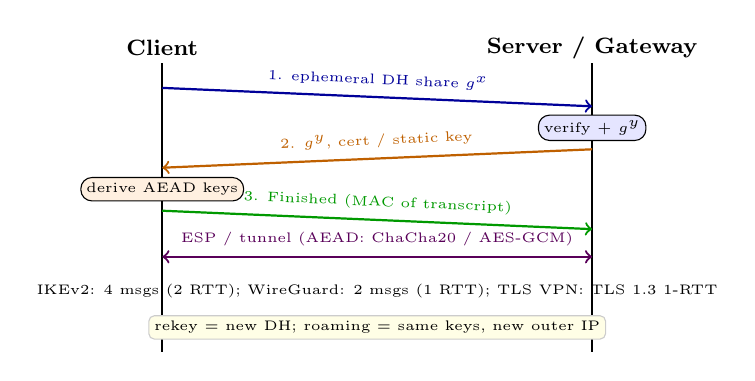
\begin{tikzpicture}[scale=0.78, every node/.style={font=\scriptsize}]
\node[font=\footnotesize\bfseries] at (1.85,5.10) {Client}; \node[font=\footnotesize\bfseries] at (8.85,5.10) {Server / Gateway};
\draw[thick] (1.85,4.85) -- (1.85,0.15); \draw[thick] (8.85,4.85) -- (8.85,0.15);
\draw[->,thick,blue!60!black] (1.85,4.45) -- (8.85,4.15) node[midway,above,sloped,font=\tiny] {1. ephemeral DH share $g^x$};
\node[draw,fill=blue!10,rounded corners,inner sep=2pt,font=\tiny] at (8.85,3.80) {verify + $g^y$};
\draw[->,thick,orange!75!black] (8.85,3.45) -- (1.85,3.15) node[midway,above,sloped,font=\tiny] {2. $g^y$, cert / static key};
\node[draw,fill=orange!12,rounded corners,inner sep=2pt,font=\tiny] at (1.85,2.80) {derive AEAD keys};
\draw[->,thick,green!60!black] (1.85,2.45) -- (8.85,2.15) node[midway,above,sloped,font=\tiny] {3. Finished (MAC of transcript)};
\draw[<->,thick,violet!70!black] (1.85,1.70) -- (8.85,1.70) node[midway,above,font=\tiny] {ESP / tunnel (AEAD: ChaCha20 / AES-GCM)};
\node[font=\tiny,align=center] at (5.35,1.15) {IKEv2: 4 msgs (2 RTT); WireGuard: 2 msgs (1 RTT); TLS VPN: TLS 1.3 1-RTT};
\node[font=\tiny,fill=yellow!10,rounded corners=2pt,inner sep=2pt,draw=gray!40] at (5.35,0.55) {rekey = new DH; roaming = same keys, new outer IP};
\end{tikzpicture}
\caption{Handshake ladder (IKEv2 / WireGuard / TLS VPN, simplified). ephemeral DH gives forward secrecy; the Finished MAC binds the transcript and prevents downgrade.}
\label{fig:handshake}
\end{figure}

\begin{table}[h]\centering\small
\begin{tabular}{l l l l}
\toprule & \textbf{IPsec} & \textbf{TLS VPN} & \textbf{WireGuard} \\ \midrule
Layer & L3 kernel, SA per flow & L4/L7 user-space & L3 kernel, cryptokey routing \\
Through NAT & Hard (ESP, NAT-T) & Easy (TCP 443) & Easy (UDP, roaming) \\
Client & Heavy (strongSwan) & Light (browser/agent) & Very light (\texttt{wg}) \\
Crypto & Agility (many suites) & TLS 1.3 suites & Fixed (Noise, ChaCha20) \\ \bottomrule
\end{tabular}
\caption{Choosing a VPN. Site-to-site on stable links favours IPsec; BYOD road warriors favour TLS VPN or WireGuard; simplicity and roaming favour WireGuard.}
\end{table}

\begin{lstlisting}[language=bash,caption={WireGuard: minimal site-to-site and client config.},label={lst:wg}]
# /etc/wireguard/wg0.conf  -- each peer is one public key + allowed IPs
[Interface]
PrivateKey = <client-private>   # Curve25519
Address = 10.8.0.2/32
DNS = 10.8.0.1                  # push private DNS to avoid leak
[Peer]  # gateway
PublicKey = <gateway-public>
AllowedIPs = 10.0.0.0/16, 10.8.0.0/24  # cryptokey routing: what goes into tunnel
Endpoint = gw.corp.example:51820
PersistentKeepalive = 25        # keep NAT mapping alive
# up: wg-quick up wg0  |  down: wg-quick down wg0
\end{lstlisting}

WireGuard's elegance is cryptokey routing: ``which packets go where'' is not
a routing table but ``which public key is allowed for which IPs.'' No
certificates, no IKE ciphers to negotiate, roaming is free because the
endpoint IP is just a hint that updates on any authenticated packet.

\begin{figure}[h]\centering
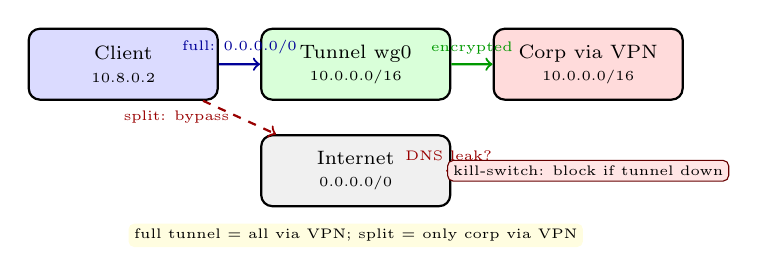
\begin{tikzpicture}[scale=0.82, every node/.style={font=\scriptsize},
  net/.style={draw,thick,rounded corners=4pt,minimum width=2.4cm,minimum height=0.90cm,align=center}]
\node[net,fill=blue!14] (client) at (0,2.10) {Client\\\tiny 10.8.0.2};
\node[net,fill=green!15] (tun) at (3.6,2.10) {Tunnel wg0\\\tiny 10.0.0.0/16};
\node[net,fill=gray!12] (inet) at (3.6,0.45) {Internet\\\tiny 0.0.0.0/0};
\node[net,fill=red!14] (corp) at (7.2,2.10) {Corp via VPN\\\tiny 10.0.0.0/16};
\draw[->,thick,blue!60!black] (client) -- (tun) node[midway,above,font=\tiny] {full: 0.0.0.0/0};
\draw[->,thick,green!60!black] (tun) -- (corp) node[midway,above,font=\tiny] {encrypted};
\draw[->,thick,red!60!black,dashed] (client) -- (inet) node[midway,left,font=\tiny] {split: bypass};
\draw[->,thick,red!60!black,dashed] (inet) -- ++(1.4,0) node[midway,above,font=\tiny] {DNS leak?};
\node[font=\tiny,fill=yellow!12,rounded corners=2pt,inner sep=2pt] at (3.6,-0.55) {full tunnel = all via VPN; split = only corp via VPN};
\node[font=\tiny,fill=red!10,rounded corners=2pt,inner sep=2pt,draw=red!40!black] at (7.2,0.45) {kill-switch: block if tunnel down};
\end{tikzpicture}
\caption{Split vs.\ full tunnel. Full tunnel protects all traffic but costs bandwidth; split saves bandwidth but must not leak DNS or IPv6 around the tunnel.}
\label{fig:split-tunnel}
\end{figure}

% ============================================================
\section{Leakage, Performance, and Policy}\label{sec:leakage}
A VPN that leaks is worse than no VPN because it creates false confidence.
Audit three leaks: \emph{DNS} (resolver bypasses tunnel), \emph{IPv6}
(tunnel is v4-only, OS prefers v6), and \emph{reconnection} (tunnel down,
traffic falls back to clear). Mitigations: push a private DNS and block
port~53 outside the tunnel, disable or tunnel IPv6, and enforce a
\emph{kill switch} (default-deny without the SA, Listing~\ref{lst:leak}).

\begin{lstlisting}[language=bash,caption={Kill-switch and leak audit (nftables + checks).},label={lst:leak}]
# nftables kill-switch: only allow out via wg0 or to the gateway
nft add rule inet filter output oifname != "wg0" ip daddr != 203.0.113.1 drop
# audit: DNS must not leave outside tunnel
tcpdump -i eth0 -n port 53 &  # should see nothing after VPN up
# audit: IPv6 must not bypass
ip -6 route | grep -v wg0 && echo "IPv6 leak!"
\end{lstlisting}

Performance: AEAD adds per-packet overhead (ESP header + tag $\approx$30--50\,B)
and crypto cost; WireGuard's ChaCha20 is fast without AES-NI, IPsec AES-GCM
is fast with it. One SA per flow (IPsec) vs.\ one interface (WireGuard) vs.\
one TLS stream (TLS VPN) changes how head-of-line blocking and rekeying
behave. Measure, do not guess: \texttt{iperf3} inside vs.\ outside the tunnel.

\begin{remark}[VPN does not replace endpoint security]\label{rem:vpn-limits}
A compromised laptop inside the tunnel is still inside the perimeter.
Combine VPN with device posture (patch level, EDR), MFA for the handshake,
and short-lived credentials. Split tunnelling (only corporate traffic via VPN)
trades bandwidth for exposure and must be policy-controlled, not user-chosen.
\end{remark}

% ============================================================
\section{Exercises}\label{sec:ch04-exercises}
\begin{enumerate}[label=E4.\arabic*, leftmargin=*, itemsep=0.6em]
    \item \textbf{Tunnel vs.\ transport.} Two gateways link \texttt{10.1.0.0/16}
    and \texttt{10.2.0.0/16} via IPsec ESP. Show the on-wire packet for
    \texttt{10.1.0.5$\to$10.2.0.9} in tunnel and in transport mode. Which hides
    the inner addresses from an observer?
    \item \textbf{Protocol choice.} A company needs (i) permanent link between two
    data centres and (ii) remote access for 500 BYOD laptops through hotel NATs.
    For each, choose IPsec vs.\ TLS VPN vs.\ WireGuard and justify with NAT
    traversal, client provisioning, and granularity.
    \item \textbf{WireGuard config.} Given Listing~\ref{lst:wg}, what happens if
    \texttt{AllowedIPs} mistakenly includes \texttt{0.0.0.0/0} on the gateway?
    What happens if \texttt{PersistentKeepalive} is omitted behind a NAT?
    \item \textbf{Leak audit.} Describe a step-by-step test that proves a VPN
    leaks DNS (record the \texttt{tcpdump} filter and expected output). Propose a
    fix via pushed DNS and a firewall rule that blocks port~53 outside the tunnel.
    \item \textbf{Performance.} ESP adds 38\,B per packet (header+IV+tag). For
    1400\,B payloads, compute overhead \%. An \texttt{iperf3} run shows 920\,Mbps
    outside, 840\,Mbps inside. Is the drop fully explained by overhead? What else
    could contribute (crypto, MTU, rekey)?
\end{enumerate}

\section*{Chapter Notes}
IPsec is RFC~4301/4303 (ESP) and RFC~7296 (IKEv2, Kaufman et~al.); TLS VPN
trade-offs follow NIST SP~800-77 Rev~1 (Frankel et~al.). WireGuard is Donenfeld,
``WireGuard: Next Generation Kernel Network Tunnel'' (NDSS 2017) and
\texttt{wireguard.com}. Comparison with TLS 1.3 handshake (Rescorla, RFC~8446)
clarifies forward secrecy. Leakage and kill-switch guidance follows Mullvad and
ANSSI hardening guides; performance numbers assume AES-GCM vs.\ ChaCha20 on
modern x86/ARM with/without AES-NI.
% End of Chapter 4
